\documentclass{article} % For LaTeX2e
\usepackage{iclr2026_conference,times}

% Minimal math_commands stub so that % Minimal math_commands stub so that % Minimal math_commands stub so that \input{math_commands.tex} resolves.
% The manuscript only relies on standard amsmath / amssymb macros.
\newcommand{\eps}{\varepsilon}
 resolves.
% The manuscript only relies on standard amsmath / amssymb macros.
\newcommand{\eps}{\varepsilon}
 resolves.
% The manuscript only relies on standard amsmath / amssymb macros.
\newcommand{\eps}{\varepsilon}


\usepackage[utf8]{inputenc}
\usepackage[T1]{fontenc}
\usepackage{microtype}

\usepackage{amsthm}
\newtheorem{claim}{Claim}
\usepackage{amsmath, amsfonts, amssymb, amsthm}
\usepackage{nicefrac}

\newtheorem{theorem}{Theorem}[section]
\newtheorem{proposition}[theorem]{Proposition}
\newtheorem{lemma}[theorem]{Lemma}
\newtheorem{definition}[theorem]{Definition}
\newtheorem{remark}[theorem]{Remark}

\usepackage{algorithm}
\usepackage{algpseudocode}

\usepackage[table]{xcolor}
\usepackage{graphicx}
\usepackage{float}
\usepackage{placeins}

\definecolor{headerpink}{RGB}{241,222,218}
\definecolor{rowgray}{RGB}{244,244,244}
\definecolor{mydarkblue}{rgb}{0,0.4,0.8}
\definecolor{mylightblue}{rgb}{0.5,0.75,1}
\definecolor{NavyBlue}{HTML}{000080}

\usepackage{booktabs}
\setlength{\heavyrulewidth}{\lightrulewidth}
\setlength{\aboverulesep}{0pt}
\setlength{\belowrulesep}{0pt}

\usepackage{enumitem}
\usepackage{pifont}
\usepackage{xspace}
\usepackage{url}

\newcommand{\XL}[1]{\textcolor{orange}{[XL: #1]}}

% Method naming: PANDA (Perturbation-based Analysis of Dissent and Hesitation)
\DeclareRobustCommand{\method}{%
  \texorpdfstring{%
    \ifmmode\text{\normalfont\textsc{panda}}\else\textsc{panda}\xspace\fi
  }{PANDA}%
}
\newcommand{\MethodFull}{\emph{Perturbation-based Analysis of Dissent and Hesitation}\xspace}
\newcommand{\Dissent}{\emph{dissent}\xspace}
\newcommand{\Hesitation}{\emph{hesitation}\xspace}

\usepackage{hyperref}
\hypersetup{
    colorlinks=true,
    linkcolor=red,
    citecolor=mydarkblue,
    filecolor=magenta,
    urlcolor=magenta,
}

\title{Beyond Self-Consistency: Perturbation-based Uncertainty Quantification\\ for LLM Reasoning via Dissent and Hesitation}

% Anonymous for double-blind review (ICLR 2026).
\author{Anonymous authors\\
Paper under double-blind review}

\newcommand{\fix}{\marginpar{FIX}}
\newcommand{\new}{\marginpar{NEW}}

%\iclrfinalcopy % Uncomment for camera-ready version, but NOT for submission.
\begin{document}

\maketitle

\begin{abstract}
Large language models (LLMs) increasingly drive high-stakes reasoning applications, yet they often fail to signal when their answers are wrong. The dominant paradigm for uncertainty quantification (UQ) estimates confidence from the dispersion of multiple sampled answers, assuming that uncertainty surfaces as output disagreement. We show that this assumption breaks down in multi-step reasoning: under multi-sampling, LLMs frequently exhibit a \emph{self-consistent collapse}, where diverse sampling trajectories converge on the same incorrect answer, yielding a highly consistent but wrong consensus. As a result, error detection based on sampling saturates quickly and leaves a stubborn residue of confident errors, an effect that intensifies as models grow more capable. To move beyond output-level statistics, we propose \method{} (\MethodFull), a UQ framework that probes the model with a joint ensemble of input rephrasings and low-rank weight perturbations. \method{} couples an answer-level \Dissent{} signal, which measures how often perturbed runs reject the base answer, with a process-level \Hesitation{} signal, which measures near-answer token entropy along the reasoning trace, and fuses them through a lightweight, out-of-fold logistic calibration. Across four open-source LLMs and multiple mathematical reasoning benchmarks, \method{} consistently outperforms strong answer-level and token-level baselines in error detection (AUROC/AUPRC) and selective accuracy, and ablations confirm that both dissent and hesitation are essential under self-consistent collapse.
\end{abstract}

\section{Introduction}
\label{sec:intro}
As large language models (LLMs) are increasingly deployed in real-world applications where reliability is critical, ensuring the trustworthiness of their outputs has become a central concern. Despite their strong performance across a wide range of reasoning tasks, LLMs often fail to reliably indicate when their predictions are uncertain. This issue is particularly pronounced in complex multi-step reasoning settings, where models may produce fluent and seemingly well-reasoned responses that are nevertheless incorrect or unsupported by the underlying problem. Such failures make it difficult to assess output reliability, even when the generated responses appear plausible.

Current approaches for uncertainty quantification in large language models can be categorized into two main paradigms. The first category consists of answer-level methods. These approaches typically rely on multiple sampling or high-temperature decoding, and characterize uncertainty by analyzing the consistency among multiple generated responses. Representative methods include self-consistency and its variants, as well as semantic entropy-based approaches, which cluster semantically equivalent outputs and compute entropy over the resulting distribution. The second category focuses on leveraging information from the generation process. These methods directly utilize token-level signals, probability distributions, or internal model states during generation to construct uncertainty quantification. Despite their differences in implementation, these two paradigms are often viewed as a dichotomy: the former operates on the output space, while the latter leverages observable signals within the generation process.

However, we find that large language models can exhibit a mode-collapsed failure mode under multi-sampling, where diverse sampling trajectories converge to the same incorrect answer, forming a highly consistent yet erroneous consensus. In such cases, the model exhibits high agreement while remaining systematically wrong, indicating a failure mode where uncertainty is not reflected in output variability. This challenges the commonly used assumption that epistemic uncertainty can be faithfully captured by dispersion across sampled outputs. In particular, while output-level variance is expected to increase with uncertainty under multi-sampling, this correspondence breaks down in complex reasoning tasks. Furthermore, we observe that increasing the number of samples improves error detection only up to a point, after which performance quickly saturates, limiting the effectiveness of additional sampling in identifying high-confidence errors. These observations suggest that the conventional answer-level approach under multi-sampling is insufficient for characterizing uncertainty in complex reasoning tasks, as errors may concentrate into highly consistent and high-confidence predictions rather than being distributed across diverse outputs, which motivates us to tap into process-level signals to extract complementary and comprehensive information for better uncertainty quantification in LLM reasoning.

Therefore, we propose \method{}, a perturbation-based uncertainty quantification framework that goes beyond standard high-temperature sampling based methods, and jointly leverages both answer-level and process-level signals for more reliable uncertainty quantification in reasoning tasks.
More specifically, \method{} constructs a set of perturbed inference trajectories through both input rephrasing and model weight perturbations, and uses their output disagreement to capture answer-level uncertainty. At the same time, it exploits token-level probability dynamics within each trajectory to measure process-level hesitation during reasoning. By integrating these complementary signals, \method{} provides a unified framework for uncertainty quantification that can better capture uncertainty in reasoning scenarios.

Our main contributions are summarized as follows:

\begin{itemize}[leftmargin=*]

\item[\ding{182}] \textit{\textbf{Failure Mode of Answer-Level UQ:}}
We identify a failure mode in multi-sampled decoding, where large language models exhibit self-consistent collapse, producing highly consistent yet incorrect predictions that violate the assumption that uncertainty is reflected in output dispersion.

\item[\ding{183}] \textit{\textbf{A New Perturbation-Based Uncertainty Framework:}}
We propose \method{}, a perturbation-based uncertainty estimation framework that constructs a joint ensemble over input rephrasing and model weight perturbations. \method{} integrates answer-level disagreement with process-level hesitation signals, enabling more reliable uncertainty estimation beyond output-level statistics.

\item[\ding{184}] \textit{\textbf{Empirical Validation:}}
We empirically evaluate \method{} across multiple reasoning benchmarks and open-source LLMs, demonstrating consistent improvements over strong baselines in uncertainty estimation and error detection. Further analysis shows that both perturbation-based disagreement and process-level signals are critical for robust performance under self-consistent collapse.

\end{itemize}

\section{Preliminaries}

In this section, we introduce the notation used throughout the paper and review the autoregressive generation process and perturbation-based inference setting underlying our method.

\paragraph{Notation.}
We denote the input question as $x$. The output of a language model is represented as
$o = (\tau, a, \mathbf{p})$, where $\tau = (y_1, \dots, y_T)$ denotes the generated reasoning trace, $a$ is the final answer, and $\mathbf{p} = \{p_t\}_{t=1}^{T}$ denotes the sequence of token-level probability distributions. We define a perturbation-induced output set as
\[
\mathcal{O}(x) = \{o_j\}_{j=1}^{K},
\]
where each output $o_j$ is generated under either input rephrasing or model weight perturbation.

We use $a_i \equiv a_j$ to denote task-specific equivalence between two final answers. For each decoding step $t$, $p_t(v)$ denotes the probability assigned to token $v$ conditioned on $x$ and the prefix $y_{<t}$. We further denote $\mathcal{M}_t$ as the set of top-$M$ tokens at step $t$.

\paragraph{Autoregressive language modeling.}
We consider a language model parameterized by $\theta$, which defines a probability distribution over token sequences conditioned on an input $x$. Given an output sequence $y = (y_1, \dots, y_T)$, the model factorizes the joint distribution as
\[
p_{\theta}(y \mid x) = \prod_{t=1}^{T} p_{\theta}(y_t \mid x, y_{<t}),
\]
where $y_{<t}$ denotes the generated prefix up to step $t$. Generation proceeds sequentially by sampling or decoding from $p_{\theta}(y_t \mid x, y_{<t})$ until a termination condition is reached. This formulation underlies standard decoding strategies such as greedy decoding and stochastic sampling.

\paragraph{Low-rank weight perturbation.}
Our perturbations act in a low-rank subspace of the model parameters and require
no additional training. Consider a pretrained weight matrix
$W_0 \in \mathbb{R}^{m \times n}$, and let $U \in \mathbb{R}^{m \times r}$ collect
the top-$r$ left singular vectors of $W_0$ (obtained by a truncated singular value
decomposition), with $r \ll \min(m,n)$. A perturbed weight is produced by
injecting noise confined to this subspace,
\[
W = W_0 + U E^\top, \qquad
E \in \mathbb{R}^{n \times r},\quad E_{ij} \sim \mathcal{N}(0, \rho^2),
\]
where $E$ is a random (non-trainable) coefficient matrix and $\rho$ controls the
perturbation strength. This defines a stochastic weight ensemble around $W_0$;
Section~\ref{sec:perturbation-ensemble} instantiates it on the attention
query/key projections.

\section{Method}

\subsection{Problem Definition}

Given an input question $x$, a large language model generates an output $o = (\tau, a, \mathbf{p})$, where $a$ is the final answer. The goal of uncertainty estimation is to learn a scoring function $S(x)$ that predicts whether the model output is correct or not, without access to ground-truth labels at inference time.

\subsection{Overview}
We propose a perturbation-based framework for estimating uncertainty in large language models. The key idea is to evaluate model behavior under controlled variations of input prompts and model parameters, and aggregate signals from both output-level disagreement and process-level instability into a unified uncertainty score.

\subsection{Perturbation Ensemble}
\label{sec:perturbation-ensemble}

\method\ builds a perturbation ensemble from two independent perspectives, text
perturbations and weight perturbations.
Text perturbations test whether the model is robust to semantic changes of the
input prompt, while weight perturbations test whether the model is robust to
small changes in its parameters.

\paragraph{Text perturbation.}
Given a question $x$, we construct $R$ input variants
$\mathcal{X}(x)=\{\tilde{x}^{(r)}\}_{r=1}^{R}$.
Each $\tilde{x}^{(r)}$ is generated by an external rephrasing under the
instruction to preserve the original problem's mathematical meaning,
constraints, and expected answer.
This gives a text-side perturbation axis that changes the surface form of the
problem while keeping the target answer unchanged.

\paragraph{Weight perturbation.}
In parallel, we construct $W$ model-side perturbations by introducing stochastic noise in a fixed set of projection matrices $\mathcal{P}$ of the base model $p_{\theta_0}$. In this work, we restrict $\mathcal{P}$ to the query and key projection matrices, i.e., $\mathcal{P} = \{W_Q, W_K\}$ across attention layers. For each selected matrix $W_\ell^0 \in \mathbb{R}^{m_\ell \times n_\ell}$ (where $\ell \in \mathcal{P}$ indexes either query or key projections), we perform a low-rank decomposition and denote $U_{\ell,r'} \in \mathbb{R}^{m_\ell \times r'}$ as the subspace spanned by the top $r'$ left singular vectors of $W_\ell^0$, where $r' \ll \min(m_\ell, n_\ell)$.

For the $w$-th perturbation, we sample a noise matrix
\[
E_{\ell}^{(w)} \in \mathbb{R}^{n_\ell \times r'}, \quad
E_{\ell,ij}^{(w)} \sim \mathcal{N}(0, \rho_\ell^2),
\]

and construct the perturbed weight as
\[
W_\ell^{(w)} = W_\ell^0 + U_{\ell,r'} (E_{\ell}^{(w)})^\top.
\]

All query and key projection matrices across all transformer layers are perturbed independently following the same procedure. All parameters outside $\mathcal{P}$ remain unchanged. Each perturbed model instance is fixed during the generation of a single response.

\paragraph{Joint perturbation.}
We first decode one \emph{base} response from the original prompt with the
unperturbed model:
\[
o_0=(\tau_0,a_0,\mathbf{p}_0),
\]
where $\tau_0=(y_{0,1},\ldots,y_{0,T_0})$ is the reasoning trace, $a_0$ is the
extracted final answer, and $\mathbf{p}_0=\{p_{0,t}\}_{t=1}^{T_0}$ stores the
retained top-$M$ token distributions along the trace.
We then merge the text and weight perturbation axes into a single ensemble of
$K=R+W$ additional responses:
\[
\mathcal{O}_{\mathrm{pert}}(x)
=
\{o_j=(\tau_j,a_j,\mathbf{p}_j)\}_{j=1}^{K}.
\]
The ensemble contains $R$ responses decoded from rephrased prompts using the
base model and $W$ responses decoded from perturbed models using the original
prompt.
Let $\mathcal{M}_{j,t}$ denote the retained top-$M$ token set at position $t$.
All \method\ signals below are computed from $a_0$ and
$\mathcal{O}_{\mathrm{pert}}(x)$; no extra generations are required beyond the
standard $1{+}K$ decoding budget used in our experiments.

\subsection{The \method\ Score}
\label{sec:panda-score}

\method\ combines two perturbation-induced signals: outcome dissent and process
hesitation.
Outcome dissent tests whether perturbed runs reject the greedy base answer,
while process hesitation tests whether the reasoning trace remains predictively
unstable near answer commitment.
We combine their standardized values into a single unreliability score:
\begin{equation}
\label{eq:panda}
S_{\mathrm{PANDA}}(x)
=
\sigma\!\left(
w_D \tilde{D}_{\mathrm{dissent}}(x)
+
w_H \tilde{H}_{\mathrm{hes}}(x)
+
b
\right).
\end{equation}
Here $\tilde{D}_{\mathrm{dissent}}(x)$ and
$\tilde{H}_{\mathrm{hes}}(x)$ denote training-fold standardized versions of the
two signals.
Both the components and the final score are oriented so that larger values
indicate lower reasoning reliability.
The calibration of $w_D,w_H$ and $b$ is described after the component
definitions.

\paragraph{Dissent.}
Dissent measures whether perturbations reject the answer produced by the greedy
base run. Let $a_0$ be the base answer and $a_j$ be the answer extracted from the
$j$-th perturbation response. We write $a_j \equiv a_0$ when the two answers are
equivalent under the task-specific answer matcher. The dissent score is
\[
D_{\mathrm{dissent}}(x)
=
\frac{1}{K}
\sum_{j=1}^{K}
\mathbf{1}\!\left[a_j \not\equiv a_0\right].
\]
This score is $0$ when every perturbation run agrees with the base answer, $1$
when all perturbation runs disagree with it, and increases in discrete steps of
$1/K$.

\paragraph{Hesitation.}
Dissent uses only hard final answers.
Hesitation instead measures process and token-level instability inside the
reasoning trace.
We estimate this instability with near-answer token entropy:
as the model approaches the final answer span, token distributions should
typically sharpen; if they remain diffuse, the trace has not yet converged.
This serves as a proxy for the model's internal hesitation before committing to
the final answer.
For each perturbation response $o_j$, let $\alpha_j$ denote the start position
of the final answer span in $\tau_j$. We assign larger weights to tokens closer to the final answer, reflecting their greater relevance to the model's commitment process.
For each pre-answer position $0 \leq t < \alpha_j$, define the linear proximity
weight $r_{j,t}=(t+1)/\alpha_j$ and the renormalized top-$M$ distribution
$\hat{p}_{j,t}(v)=p_{j,t}(v)/\sum_{u\in\mathcal{M}_{j,t}}p_{j,t}(u)$.
The question-level hesitation score is
\[
H_{\mathrm{hes}}(x)
=
\frac{1}{K}
\sum_{j=1}^{K}
\frac{
\sum_{t=0}^{\alpha_j-1}
r_{j,t}
\left[
-\sum_{v\in\mathcal{M}_{j,t}}
\hat{p}_{j,t}(v)\log \hat{p}_{j,t}(v)
\right]
}{
\sum_{t=0}^{\alpha_j-1} r_{j,t}
}.
\]
We compute hesitation on perturbation runs only; the base trace supplies the
anchor answer $a_0$ but is not averaged into $H_{\mathrm{hes}}$.

\paragraph{Calibration.}
The weights $w_D,w_H$ and bias $b$ in Eq.~\ref{eq:panda} are learned by a
lightweight logistic calibration.
During evaluation, calibration follows a leave-one-dataset-out protocol: when
scoring a held-out dataset $D_i$, all standardization statistics, median
imputation values, and calibration parameters are estimated only from the
remaining datasets.
Thus, $S_{\mathrm{PANDA}}(x)$ is always reported out of fold, with no labels from
the evaluated dataset used to fit the score.
At deployment, the same calibration can be fit once on a separate held-out
calibration pool.
A larger $S_{\mathrm{PANDA}}(x)$ indicates lower reasoning reliability, and the
score is used directly for uncertainty ranking and error detection.

\section{Experiments}

We evaluate \method\ as an answer-level reliability score for reasoning
responses.
The goal is to determine whether an unreliability score can distinguish
incorrect answers from correct ones without access to ground-truth labels at
test time.
We first compare \method\ with strong uncertainty-quantification baselines, and
then analyze whether dissent and hesitation reveal complementary process-level
failure patterns.

\subsection{Experimental Setup}
\label{sec:experimental-setup}

\paragraph{Datasets.}
Our main experiments are conducted on three mathematical reasoning benchmarks: GSM8K, MATH-500, and Minerva, covering grade-school word problems, competition-level mathematics, and advanced reasoning tasks respectively. For the analysis experiments, DeepScaleR, GPQA, and AIME 2024 are used.

\paragraph{Models.}
For the main experiments, we evaluate four open-source instruction-tuned models: Qwen2.5-3B, Llama-3.2-1B, Llama-3.1-8B, and Qwen3-8B. For the analysis experiments, Qwen2.5-0.5B, Llama-3.2-1B, Qwen2.5-1.5B, Phi-4-mini, Qwen2.5-3B, and Qwen2.5-7B are used. All models are served with vLLM in bfloat16 precision.

\paragraph{Baselines.}
We systematically categorize our baselines into two distinct types:
(i) those relying solely on the target model's internal process-level signals, including P(True), Predictive Entropy (PE), Log-Likelihood (LL), Self-Certainty, Deep Think with Confidence (DeepConf), and token-level uncertainty with epistemic estimation (TokUR EU); and
(ii) those leveraging external signals, such as an auxiliary Natural Language Inference (NLI) model or semantic-similarity graph: Semantic Entropy (SE), Eccentricity (Ecc), Degree Matrix (Deg), and Shifting Attention to Relevance (SAR).

\paragraph{Metrics.}
We evaluate uncertainty estimation using AUROC and AUPRC for error detection, treating incorrect answers as the positive class. For the main experiments, we additionally report selective accuracy at 50\% coverage (Acc@50). For the analysis experiments, we further report the Confident Wrong rate (CW@$\tau$) and stability across sampling budgets $n \in \{2,4,8,16,32,64\}$.

\subsection{Failure Mode Analysis}

We evaluate answer-level uncertainty quantification under multi-sampled decoding across multiple reasoning benchmarks and open-source models. As shown in Figure~\ref{fig:answer-uq-limit}, increasing the number of sampled responses improves error detection performance in low-sample regimes, as measured by AUROC, but the gain quickly saturates across all evaluated models. We further observe that a non-negligible fraction of incorrect predictions remains highly consistent under sampling, concentrating on the same erroneous answer with high confidence (e.g., $p_{\mathrm{top}} \ge 0.9$). This indicates that output-level dispersion is insufficient to fully capture uncertainty in such cases. Moreover, this failure mode becomes more pronounced as model capability increases, where incorrect predictions are more likely to manifest as highly concentrated collapses rather than dispersed errors. Overall, these results show that increasing sampling alone is insufficient to reliably improve answer-level uncertainty quantification in complex reasoning tasks.
\begin{figure}[htbp]
    \centering
    \includegraphics[width=\linewidth]{iclr2026/confidentwrong.png}
    \caption{
    Answer-level UQ saturates with sampling but cannot eliminate confident wrongs.
    We evaluate six open-source models on questions from three reasoning benchmarks, drawing up to $K{=}64$ final answers per question.
    Uncertainty is $u_{\mathrm{ans}}(x;n)=1-p_{\mathrm{top}}(x;n)$.
    (a) AUROC for detecting majority errors rises quickly at small $n$ and then saturates.
    (b) The fraction of wrong predictions with $p_{\mathrm{top}}\ge 0.9$ (CW@0.9) drops with $n$ but remains nonzero.
    (c) At $n{=}64$, the confident-wrong fraction among wrong predictions increases with model capability.
    }
    \label{fig:answer-uq-limit}
\end{figure}

\subsection{Main Results}
\label{sec:main-results}

% Put these before the table, e.g., in the preamble or right before the table.
\newcommand{\metric}[2]{{\large #1} $\pm$ {\scriptsize #2}}
\newcommand{\bestmetric}[2]{\textbf{{\large #1}} $\pm$ {\scriptsize #2}}

\begin{table*}[t]
  \centering
  \small
  \setlength{\tabcolsep}{5.0pt}
  \renewcommand{\arraystretch}{1.12}
  \caption{
  Metrics are AUROC / AUPRC / Acc@50 under clean labels, with incorrect answers
  as the positive class.
  Values are mean $\pm$ std over three seeds on the clean evaluated cohort
  ($N{=}8121$).
  Best results in each column are bold.
}
  \label{tab:main-all-baselines}
  \resizebox{\textwidth}{!}{
  \begin{tabular}{l|ccc|ccc|ccc}
    \toprule
    \rowcolor{headerpink}
    & \multicolumn{3}{c|}{Minerva}
    & \multicolumn{3}{c|}{MATH-500}
    & \multicolumn{3}{c}{GSM8K} \\
    \rowcolor{headerpink}
    Method
    & AUROC & AUPRC & ACC*
    & AUROC & AUPRC & ACC*
    & AUROC & AUPRC & ACC* \\
    \midrule

    \multicolumn{10}{l}{\textbf{Qwen2.5-3B}} \\
    SE
      & \metric{0.638}{0.026} & \metric{0.716}{0.022} & \metric{0.513}{0.030}
      & \metric{0.709}{0.007} & \metric{0.442}{0.034} & \metric{0.878}{0.008}
      & \metric{0.613}{0.023} & \metric{0.169}{0.046} & \metric{0.958}{0.003} \\
    \rowcolor{rowgray}
    Ecc
      & \metric{0.493}{0.038} & \metric{0.595}{0.038} & \metric{0.406}{0.032}
      & \metric{0.580}{0.011} & \metric{0.271}{0.006} & \metric{0.829}{0.010}
      & \metric{0.585}{0.080} & \metric{0.129}{0.044} & \metric{0.947}{0.011} \\
    Deg
      & \metric{0.657}{0.047} & \metric{0.730}{0.029} & \metric{0.513}{0.046}
      & \metric{0.758}{0.011} & \metric{0.484}{0.030} & \metric{0.908}{0.019}
      & \metric{0.663}{0.030} & \metric{0.211}{0.009} & \metric{0.962}{0.003} \\
    \rowcolor{rowgray}
    SAR
      & \metric{0.617}{0.019} & \metric{0.716}{0.017} & \metric{0.463}{0.007}
      & \metric{0.601}{0.033} & \metric{0.414}{0.025} & \metric{0.783}{0.019}
      & \metric{0.461}{0.013} & \metric{0.089}{0.017} & \metric{0.913}{0.011} \\
    PE
      & \metric{0.663}{0.016} & \metric{0.748}{0.019} & \metric{0.486}{0.016}
      & \metric{0.592}{0.030} & \metric{0.401}{0.017} & \metric{0.763}{0.028}
      & \metric{0.477}{0.013} & \metric{0.113}{0.001} & \metric{0.922}{0.009} \\
    \rowcolor{rowgray}
    LL
      & \metric{0.638}{0.017} & \metric{0.713}{0.019} & \metric{0.480}{0.019}
      & \metric{0.587}{0.030} & \metric{0.389}{0.017} & \metric{0.769}{0.025}
      & \metric{0.473}{0.015} & \metric{0.070}{0.002} & \metric{0.924}{0.012} \\
    Self-Certainty
      & \metric{0.662}{0.016} & \metric{0.748}{0.019} & \metric{0.486}{0.016}
      & \metric{0.592}{0.030} & \metric{0.401}{0.017} & \metric{0.769}{0.025}
      & \metric{0.477}{0.013} & \metric{0.105}{0.012} & \metric{0.922}{0.009} \\
    \rowcolor{rowgray}
    DeepConf
      & \metric{0.694}{0.010} & \metric{0.757}{0.007} & \metric{0.520}{0.018}
      & \metric{0.651}{0.038} & \metric{0.454}{0.034} & \metric{0.810}{0.022}
      & \metric{0.574}{0.037} & \metric{0.100}{0.010} & \metric{0.933}{0.010} \\
    TokUR EU
      & \metric{0.805}{0.000} & \bestmetric{0.952}{0.001} & \metric{0.587}{0.006}
      & \metric{0.725}{0.026} & \metric{0.763}{0.030} & \metric{0.644}{0.029}
      & \metric{0.711}{0.011} & \metric{0.292}{0.042} & \metric{0.935}{0.011} \\
    \rowcolor{rowgray}
    \method\ (Ours)
      & \bestmetric{0.865}{0.013} & \metric{0.915}{0.009} & \bestmetric{0.673}{0.024}
      & \bestmetric{0.934}{0.005} & \bestmetric{0.807}{0.033} & \bestmetric{0.975}{0.000}
      & \bestmetric{0.788}{0.019} & \bestmetric{0.629}{0.033} & \bestmetric{0.967}{0.000} \\

    \midrule

    \multicolumn{10}{l}{\textbf{Llama-3.2-1B}} \\
    SE
      & \metric{0.564}{0.030} & \metric{0.918}{0.012} & \metric{0.121}{0.020}
      & \metric{0.610}{0.035} & \metric{0.711}{0.016} & \metric{0.457}{0.039}
      & \metric{0.617}{0.009} & \metric{0.514}{0.004} & \metric{0.676}{0.019} \\
    \rowcolor{rowgray}
    Ecc
      & \metric{0.529}{0.033} & \metric{0.896}{0.020} & \metric{0.121}{0.018}
      & \metric{0.596}{0.016} & \metric{0.703}{0.006} & \metric{0.444}{0.042}
      & \metric{0.551}{0.004} & \metric{0.448}{0.006} & \metric{0.613}{0.014} \\
    Deg
      & \metric{0.577}{0.031} & \metric{0.919}{0.006} & \metric{0.133}{0.021}
      & \metric{0.642}{0.028} & \metric{0.735}{0.028} & \metric{0.434}{0.017}
      & \metric{0.670}{0.003} & \metric{0.559}{0.009} & \metric{0.728}{0.013} \\
    \rowcolor{rowgray}
    SAR
      & \metric{0.634}{0.020} & \metric{0.925}{0.007} & \metric{0.153}{0.005}
      & \metric{0.549}{0.012} & \metric{0.710}{0.012} & \metric{0.335}{0.014}
      & \metric{0.551}{0.004} & \metric{0.495}{0.013} & \metric{0.597}{0.011} \\
    PE
      & \metric{0.637}{0.022} & \metric{0.927}{0.006} & \metric{0.160}{0.019}
      & \metric{0.542}{0.011} & \metric{0.705}{0.011} & \metric{0.332}{0.013}
      & \metric{0.549}{0.004} & \metric{0.489}{0.011} & \metric{0.595}{0.008} \\
    \rowcolor{rowgray}
    LL
      & \metric{0.630}{0.025} & \metric{0.925}{0.008} & \metric{0.153}{0.014}
      & \metric{0.534}{0.012} & \metric{0.699}{0.012} & \metric{0.326}{0.013}
      & \metric{0.546}{0.004} & \metric{0.484}{0.011} & \metric{0.591}{0.016} \\
    Self-Certainty
      & \metric{0.631}{0.022} & \metric{0.926}{0.006} & \metric{0.157}{0.018}
      & \metric{0.538}{0.011} & \metric{0.700}{0.012} & \metric{0.335}{0.014}
      & \metric{0.546}{0.004} & \metric{0.487}{0.011} & \metric{0.593}{0.008} \\
    \rowcolor{rowgray}
    DeepConf
      & \metric{0.721}{0.018} & \metric{0.948}{0.001} & \metric{0.168}{0.024}
      & \metric{0.618}{0.009} & \metric{0.744}{0.008} & \metric{0.432}{0.007}
      & \metric{0.598}{0.005} & \metric{0.553}{0.012} & \metric{0.629}{0.019} \\
    TokUR EU
      & \metric{0.752}{0.051} & \bestmetric{0.979}{0.004} & \metric{0.094}{0.000}
      & \metric{0.783}{0.038} & \bestmetric{0.934}{0.008} & \metric{0.331}{0.035}
      & \metric{0.758}{0.006} & \metric{0.795}{0.027} & \metric{0.642}{0.064} \\
    \rowcolor{rowgray}
    \method\ (Ours)
      & \bestmetric{0.757}{0.040} & \metric{0.954}{0.013} & \bestmetric{0.179}{0.009}
      & \bestmetric{0.844}{0.012} & \metric{0.900}{0.012} & \bestmetric{0.571}{0.008}
      & \bestmetric{0.896}{0.009} & \bestmetric{0.860}{0.019} & \bestmetric{0.895}{0.003} \\

    \midrule

    \multicolumn{10}{l}{\textbf{Llama-3.1-8B}} \\
    SE
      & \metric{0.582}{0.002} & \metric{0.710}{0.013} & \metric{0.410}{0.021}
      & \metric{0.659}{0.011} & \metric{0.493}{0.007} & \metric{0.743}{0.006}
      & \metric{0.632}{0.037} & \metric{0.223}{0.032} & \metric{0.933}{0.014} \\
    \rowcolor{rowgray}
    Ecc
      & \metric{0.464}{0.031} & \metric{0.633}{0.018} & \metric{0.317}{0.008}
      & \metric{0.518}{0.023} & \metric{0.393}{0.028} & \metric{0.653}{0.027}
      & \metric{0.618}{0.006} & \metric{0.175}{0.019} & \metric{0.936}{0.006} \\
    Deg
      & \metric{0.587}{0.012} & \metric{0.716}{0.011} & \metric{0.403}{0.015}
      & \metric{0.715}{0.027} & \metric{0.546}{0.040} & \metric{0.792}{0.013}
      & \metric{0.749}{0.025} & \metric{0.305}{0.037} & \metric{0.953}{0.009} \\
    \rowcolor{rowgray}
    SAR
      & \metric{0.646}{0.017} & \metric{0.787}{0.013} & \metric{0.402}{0.014}
      & \metric{0.575}{0.007} & \metric{0.543}{0.007} & \metric{0.642}{0.003}
      & \metric{0.574}{0.015} & \metric{0.186}{0.018} & \metric{0.933}{0.000} \\
    PE
      & \metric{0.635}{0.015} & \metric{0.780}{0.010} & \metric{0.395}{0.018}
      & \metric{0.582}{0.008} & \metric{0.554}{0.008} & \metric{0.639}{0.013}
      & \metric{0.569}{0.016} & \metric{0.186}{0.031} & \metric{0.933}{0.000} \\
    \rowcolor{rowgray}
    LL
      & \metric{0.630}{0.012} & \metric{0.773}{0.005} & \metric{0.395}{0.018}
      & \metric{0.566}{0.009} & \metric{0.525}{0.017} & \metric{0.621}{0.007}
      & \metric{0.568}{0.017} & \metric{0.175}{0.035} & \metric{0.935}{0.003} \\
    Self-Certainty
      & \metric{0.634}{0.015} & \metric{0.779}{0.010} & \metric{0.395}{0.018}
      & \metric{0.573}{0.009} & \metric{0.542}{0.009} & \metric{0.636}{0.009}
      & \metric{0.569}{0.016} & \metric{0.186}{0.031} & \metric{0.933}{0.000} \\
    \rowcolor{rowgray}
    DeepConf
      & \metric{0.686}{0.011} & \metric{0.830}{0.006} & \metric{0.409}{0.022}
      & \metric{0.694}{0.007} & \metric{0.662}{0.029} & \metric{0.714}{0.024}
      & \metric{0.760}{0.015} & \metric{0.251}{0.029} & \metric{0.982}{0.006} \\
    TokUR EU
      & \metric{0.766}{0.020} & \metric{0.842}{0.006} & \metric{0.475}{0.012}
      & \metric{0.772}{0.029} & \bestmetric{0.866}{0.012} & \metric{0.640}{0.041}
      & \metric{0.851}{0.018} & \metric{0.611}{0.040} & \metric{0.969}{0.008} \\
    \rowcolor{rowgray}
    \method\ (Ours)
      & \bestmetric{0.767}{0.014} & \bestmetric{0.852}{0.022} & \bestmetric{0.491}{0.003}
      & \bestmetric{0.899}{0.002} & \metric{0.860}{0.013} & \bestmetric{0.890}{0.015}
      & \bestmetric{0.873}{0.005} & \bestmetric{0.667}{0.018} & \bestmetric{0.987}{0.000} \\

    \midrule

    \multicolumn{10}{l}{\textbf{Qwen3-8B}} \\
    SE
      & \metric{0.649}{0.014} & \metric{0.571}{0.005} & \metric{0.662}{0.044}
      & \metric{0.608}{0.036} & \metric{0.151}{0.025} & \metric{0.920}{0.007}
      & \metric{0.559}{0.026} & \metric{0.081}{0.010} & \metric{0.953}{0.000} \\
    \rowcolor{rowgray}
    Ecc
      & \metric{0.557}{0.049} & \metric{0.479}{0.038} & \metric{0.570}{0.054}
      & \metric{0.524}{0.038} & \metric{0.107}{0.012} & \metric{0.907}{0.010}
      & \metric{0.539}{0.022} & \metric{0.064}{0.008} & \metric{0.946}{0.000} \\
    Deg
      & \metric{0.704}{0.010} & \metric{0.617}{0.011} & \bestmetric{0.706}{0.014}
      & \metric{0.653}{0.021} & \metric{0.179}{0.022} & \metric{0.941}{0.010}
      & \metric{0.580}{0.023} & \metric{0.100}{0.018} & \metric{0.951}{0.003} \\
    \rowcolor{rowgray}
    SAR
      & \metric{0.650}{0.011} & \metric{0.841}{0.002} & \metric{0.399}{0.047}
      & \metric{0.773}{0.027} & \metric{0.668}{0.021} & \metric{0.889}{0.009}
      & \metric{0.795}{0.022} & \metric{0.621}{0.028} & \metric{0.883}{0.020} \\
    PE
      & \metric{0.694}{0.019} & \metric{0.860}{0.007} & \metric{0.428}{0.030}
      & \metric{0.784}{0.026} & \metric{0.680}{0.013} & \metric{0.889}{0.001}
      & \metric{0.806}{0.023} & \metric{0.636}{0.031} & \metric{0.887}{0.023} \\
    \rowcolor{rowgray}
    LL
      & \metric{0.691}{0.020} & \metric{0.859}{0.006} & \metric{0.427}{0.018}
      & \metric{0.785}{0.025} & \metric{0.659}{0.016} & \metric{0.889}{0.001}
      & \metric{0.800}{0.023} & \metric{0.620}{0.041} & \metric{0.887}{0.023} \\
    Self-Certainty
      & \metric{0.694}{0.019} & \metric{0.860}{0.007} & \metric{0.428}{0.030}
      & \metric{0.784}{0.026} & \metric{0.681}{0.013} & \metric{0.889}{0.001}
      & \metric{0.806}{0.023} & \metric{0.635}{0.031} & \metric{0.887}{0.023} \\
    \rowcolor{rowgray}
    DeepConf
      & \metric{0.682}{0.023} & \metric{0.856}{0.006} & \metric{0.439}{0.030}
      & \metric{0.764}{0.030} & \metric{0.671}{0.013} & \metric{0.864}{0.004}
      & \metric{0.834}{0.016} & \metric{0.686}{0.023} & \metric{0.902}{0.001} \\
    TokUR EU
      & \metric{0.706}{0.020} & \metric{0.821}{0.021} & \metric{0.401}{0.006}
      & \metric{0.806}{0.003} & \metric{0.774}{0.030} & \metric{0.724}{0.044}
      & \metric{0.781}{0.173} & \metric{0.391}{0.133} & \metric{0.847}{0.157} \\
    \rowcolor{rowgray}
    \method\ (Ours)
      & \bestmetric{0.926}{0.026} & \bestmetric{0.944}{0.036} & \metric{0.562}{0.016}
      & \bestmetric{0.984}{0.000} & \bestmetric{0.958}{0.004} & \bestmetric{1.000}{0.000}
      & \bestmetric{0.966}{0.003} & \bestmetric{0.943}{0.008} & \bestmetric{0.985}{0.000} \\

    \bottomrule
  \end{tabular}
  }
\end{table*}

\paragraph{Main Results.}
Table~\ref{tab:main-all-baselines} reports the performance of \method{} and competing uncertainty estimation methods across four target LLMs and three mathematical reasoning benchmarks. The results show that
(1) \method{} achieves the strongest overall performance across models and benchmarks. This suggests that perturbation-based dissent and process-level hesitation provide a more general reliability signal for mathematical reasoning.
(2) Answer-level uncertainty methods that rely on NLI-based response comparison, such as SE, Ecc, Deg, and SAR, exhibit unstable performance across different models and datasets.
(3) Token-level uncertainty methods are generally stronger than purely answer-level methods, suggesting that generation-time probability dynamics contain useful information about reasoning reliability. Among them, TokUR EU is the strongest token-level baseline, as it further incorporates perturbation-induced token evidence.

\subsection{Component Ablation}
\label{sec:ablation}

\begin{table}[t]
  \centering
  \small
  \setlength{\tabcolsep}{5.5pt}
  \renewcommand{\arraystretch}{1.15}
  \caption{
    Ablation studies of our proposed \method{}.
    AUROC and AUPRC are averaged over three mathematical benchmarks on the
    pooled cohort.
  }
  \label{tab:ablation}
\resizebox{\textwidth}{!}{
  \begin{tabular}{lcccccc}
    \toprule
    \rowcolor{headerpink}
    \textbf{Metric}
    & \textbf{\method{}}
    & \textbf{ w/o Dissent}
    & \textbf{ w/o Hesitation}
    & \textbf{ w/o Text Pert.}
    & \textbf{ w/o Weight Pert.}
    & \textbf{ w/o Fusion} \\
    \midrule

    \rowcolor{rowgray}
    AUROC
    & \textbf{0.904}
    & 0.704
    & 0.897
    & 0.862
    & 0.871
    & 0.877 \\

    AUPRC
    & \textbf{0.875}
    & 0.622
    & 0.850
    & 0.789
    & 0.829
    & 0.875 \\

    \bottomrule
  \end{tabular}
  }
\end{table}

\paragraph{Ablation Studies.}
To evaluate the contribution of each component in \method{}, we introduce five ablation variants:
(1) \method{} w/o Dissent, which removes perturbation-induced final-answer disagreement;
(2) \method{} w/o Hesitation, which removes near-answer token-level hesitation;
(3) \method{} w/o Text Pert., which removes input rephrasing and keeps only model-side perturbations;
(4) \method{} w/o Weight Pert., which removes model weight perturbations and keeps only text-side perturbations; and
(5) \method{} w/o Fusion, which replaces the learned logistic fusion of dissent and hesitation with a direct unweighted summation.
The results show that
(i) removing Dissent causes the largest drop, reducing AUROC from 0.904 to 0.704 and AUPRC from 0.875 to 0.622, indicating that perturbation-induced answer disagreement is the dominant signal in \method{};
(ii) removing Hesitation leads to a smaller but consistent degradation, suggesting that near-answer token uncertainty provides complementary process-level information beyond final-answer disagreement;
(iii) removing either text or weight perturbations also hurts performance, showing that prompt-side robustness and model-side sensitivity capture different aspects of reasoning reliability;
and (iv) replacing learned fusion with direct summation reduces AUROC from 0.904 to 0.877 while leaving AUPRC unchanged, suggesting that learned fusion mainly improves the global ranking separation between correct and incorrect answers.
Overall, these results show that \method{} is primarily driven by perturbation-induced dissent, while hesitation, dual perturbation sources, and learned fusion provide complementary refinements for stable uncertainty estimation.

\subsection{Case Analysis}

\section{Related Work}

\section{Conclusion}

We revisited uncertainty quantification for LLM reasoning and identified a self-consistent collapse failure mode, in which multi-sampled decoding produces highly consistent yet incorrect answers, causing answer-level UQ to saturate and leave a residue of confident errors that grows with model capability. Motivated by this observation, we proposed \method{}, a perturbation-based framework that probes the model with a joint ensemble of input rephrasings and low-rank weight perturbations and fuses an answer-level dissent signal with a process-level hesitation signal through a lightweight, out-of-fold calibration. Across four open-source LLMs and multiple mathematical reasoning benchmarks, \method{} consistently improves error detection and selective accuracy over strong answer-level and token-level baselines, and our ablations confirm that both dissent and hesitation are necessary. Limitations include the additional decoding cost of the perturbation ensemble and an evaluation focused on mathematical reasoning; extending \method{} to open-ended generation and designing more efficient perturbation schemes are promising directions for future work.

\newpage

\appendix

\section{Implementation Details}
\label{app:impl}

Table~\ref{tab:impl-hyper} summarizes the hyperparameters used in all main experiments ($N{=}8121$).
Unless noted otherwise, every \method{} decode uses greedy decoding
($\texttt{temperature}{=}0$, $\texttt{do\_sample}{=}\texttt{false}$).
The base response and all $R{+}W$ perturbation responses share this setting; only the Semantic Entropy (SE) baseline uses stochastic decoding.

\paragraph{Perturbation budget.}
We use $R{=}4$ text rephrasings and $W{=}4$ weight perturbations, for a matched perturbation budget of $K{=}8$ additional responses plus one greedy base run ($\sim$9 decodes per question).
Each weight instance is drawn independently with seeds $\{42,43,44,45\}$ (see \texttt{scripts/run\_maintable\_3seed.sh}).

\paragraph{Weight perturbation.}
Low-rank Gaussian noise is injected into all query and key projection matrices ($\mathcal{P}=\{\mathrm{q\_proj},\mathrm{k\_proj}\}$ across layers) with rank $r'{=}4$ and scale $\sigma{=}0.03$.
Perturbed weights are fixed for the duration of a single generation and restored before the next perturbation seed is applied.

\paragraph{Process trace.}
For hesitation, we retain the top-$M{=}10$ log-probability tokens at each pre-answer position and renormalize before computing entropy.
The answer span start $\alpha_j$ is defined in Appendix~\ref{app:answer}.

\paragraph{Calibration protocol.}
Dissent and hesitation are $z$-scored within each training fold of a leave-one-dataset-out (LODO) protocol over \{Minerva, MATH-500, GSM8K\}.
A logistic regressor learns $(w_D,w_H,b)$ in Eq.~\ref{eq:panda} on the training folds only; test metrics are reported on the held-out dataset.
The w/o Fusion ablation replaces this step with an unweighted sum of standardized components.
Table~\ref{tab:lodo-calib} reports macro LODO AUROC on the pooled cohort and the bd$=0$ collapse proxy.

\begin{table}[t]
  \centering
  \small
  \caption{Main-experiment hyperparameters.}
  \label{tab:impl-hyper}
  \begin{tabular}{ll}
    \toprule
    Parameter & Value \\
    \midrule
    Text rephrases ($R$) & 4 \\
    Weight perturbations ($W$) & 4 \\
    Weight noise rank ($r'$) & 4 \\
    Weight noise scale ($\sigma$) & 0.03 \\
    Perturbed projection set & q\_proj, k\_proj (all layers) \\
    Top-$M$ tokens for hesitation & 10 \\
    Max new tokens & 2048 \\
    Base / perturb decoding & greedy ($T{=}0$) \\
    SE baseline samples / temperature & 8 / 0.5 \\
    Evaluation seeds & 41, 42, 43 \\
    Precision & bfloat16 (vLLM / HF TFB) \\
    \bottomrule
  \end{tabular}
\end{table}

\begin{table}[t]
  \centering
  \small
  \caption{LODO macro AUROC by subset (calibration folds over math datasets).}
  \label{tab:lodo-calib}
  \begin{tabular}{lrrrrr}
    \toprule
    Subset & $n$ & \method{} & bd & hes & SE \\
    \midrule
    All      & 8121 & 0.904 & 0.897 & 0.704 & 0.890 \\
    bd$=0$   & 2960 & 0.623 & 0.500 & 0.623 & 0.708 \\
    bd$=0$ wrong & 96 & --- & --- & --- & --- \\
    \bottomrule
  \end{tabular}
\end{table}


\section{Prompt Templates}
\label{app:prompts}

\paragraph{Reasoning prompts.}
Math problems use chat templates aligned with the TokUR greedy baseline (\texttt{src/panda/grading/tokur\_records.py}).
For Qwen-family models we prepend a short system role and append a boxed-answer instruction to the user turn; for Llama-family models we use the TokUR step-by-step system prompt with the raw problem as the user message.

\begin{table}[t]
  \centering
  \small
  \caption{Generation prompt templates (math benchmarks).}
  \label{tab:prompt-templates}
  \begin{tabular}{p{0.12\linewidth}p{0.82\linewidth}}
    \toprule
    Model family & Template \\
    \midrule
    Qwen &
    \textbf{System:} ``You are Qwen, created by Alibaba Cloud. You are a helpful assistant.''\\
    &
    \textbf{User:} \texttt{\{problem\} Let's think step by step and output the final answer within \textbackslash boxed\{\}.} \\
    \addlinespace
    Llama &
    \textbf{System:} TokUR math system prompt (step-by-step format ending in \verb|\boxed{answer}|).\\
    &
    \textbf{User:} \texttt{\{problem\}} \\
    \bottomrule
  \end{tabular}
\end{table}

\paragraph{API rephrasing.}
Text perturbations are produced offline by an OpenAI-compatible chat API (\texttt{src/panda/token\_qaac/api\_rephrase.py}) before inference.
The rephrase model is instructed to preserve all mathematical conditions, avoid hints or solutions, and change surface wording only.
We sample rewrites at API temperature $0.8$ with $\texttt{top\_p}{=}0.95$ and deduplicate against the original question and prior rewrites.

\begin{quote}
\small
\textbf{Rephrase system prompt.} ``Rewrite the following math problem into a semantically equivalent version.

Requirements:
1. Preserve all mathematical conditions exactly.
2. Do not solve the problem.
3. Do not add hints.
4. Do not change the final answer.
5. Change the wording, sentence structure, or order of conditions when possible.
6. Output only the rewritten problem.''

\textbf{User turn.} ``Problem:\textbackslash n\{original question\}''
\end{quote}


\section{Answer Extraction and Correctness Labeling}
\label{app:answer}

\paragraph{Answer span $\alpha_j$.}
For each generated trace $\tau_j$, we locate the final-answer span as follows.
If the response contains \verb|\boxed{...}|, $\alpha_j$ is the index of the first token overlapping the opening brace; tokens before $\alpha_j$ contribute to hesitation.
If no box is found, we approximate the answer region with the last eight generated tokens.

\paragraph{Answer matching and clean labels.}
Extracted answers are normalized with the dataset-specific grader used throughout our pipeline (Qwen math parser + \texttt{strip\_string} for competition-style sets; string/code graders for logic tasks).
Correctness labels use \emph{clean} grading (\texttt{is\_correct\_clean}): symbolic simplification and numeric tolerance are applied before comparing to the reference, which matters especially on Minerva-style free-form derivations.
All detection metrics treat incorrect answers as the positive class.


\section{Algorithm Pseudocode}
\label{app:algorithm}

\begin{algorithm}[t]
  \caption{\method{} inference and scoring (per question).}
  \label{alg:panda}
  \begin{algorithmic}[1]
    \State Decode one greedy base response $o_0=(\tau_0,a_0,\mathbf{p}_0)$ from the original prompt
    \State Generate $R$ rephrased prompts and decode one greedy response per rephrase with the base model
    \For{$w=1$ to $W$}
      \State Inject low-rank noise into $\mathcal{P}$; decode one greedy response; restore base weights
    \EndFor
    \State Compute dissent $D_{\mathrm{dissent}}$ from final-answer agreement with $a_0$
    \State Compute hesitation $H_{\mathrm{hes}}$ from top-$M$ token traces of perturbation runs
    \State \textbf{LODO calibration:} z-score $(D_{\mathrm{dissent}},H_{\mathrm{hes}})$ on training folds; logistic fuse $\rightarrow S_{\mathrm{PANDA}}$
  \end{algorithmic}
\end{algorithm}


\section{Per-Model Detection Results}
\label{app:per-model}

Table~\ref{tab:app-per-model} reports macro-averaged AUROC on the three math benchmarks for each evaluated model (mean over seeds and datasets within model; $N{=}8121$ pooled).
The full cell-level table with AUPRC and Acc@50 appears in Table~\ref{tab:main-all-baselines} of the main text.

\begin{table}[t]
  \centering
  \small
  \caption{Per-model \method{} AUROC on Minerva / MATH-500 / GSM8K (mean $\pm$ std over three seeds).}
  \label{tab:app-per-model}
  \begin{tabular}{lccc}
    \toprule
    Model & Minerva & MATH-500 & GSM8K \\
    \midrule
    Qwen2.5-3B  & $0.838 \pm 0.014$ & $0.934 \pm 0.010$ & $0.786 \pm 0.019$ \\
    Llama-3.2-1B & $0.733 \pm 0.026$ & $0.842 \pm 0.009$ & $0.896 \pm 0.009$ \\
    Llama-3.1-8B & $0.771 \pm 0.002$ & $0.893 \pm 0.003$ & $0.872 \pm 0.006$ \\
    Qwen3-8B    & $0.928 \pm 0.022$ & $0.986 \pm 0.003$ & $0.929 \pm 0.053$ \\
    \bottomrule
  \end{tabular}
\end{table}


\section{Subset Analysis}
\label{app:subsets}

Table~\ref{tab:app-subsets} reports leave-one-dataset-out AUROC on three subsets of the pooled math cohort.
The \textbf{bd$=0$} subset ($n{=}2960$) contains questions where every perturbation run agrees with the greedy base answer; here dissent is uninformative by construction (AUROC$=0.5$).
On this subset, Semantic Entropy remains stronger than \method{} (0.708 vs.\ 0.623), because no answer-level drift is observable and hesitation supplies only partial coverage (+0.123 AUROC over bd alone).
On the full set ($n{=}8121$), \method{} reaches 0.904 AUROC, driven primarily by perturbation-induced answer drift on the bd$>0$ majority ($n{=}5161$).
Text-agreement collapse proxies shrink wrong rates from 8.1\% (text\_agree) to 3.2\% (bd$=0$), leaving $n{=}96$ hard cases where every perturbation agrees with a wrong base answer.

\begin{table}[t]
  \centering
  \small
  \caption{LODO AUROC by subset ($N{=}8121$ math cohort).}
  \label{tab:app-subsets}
  \begin{tabular}{lrrrrr}
    \toprule
    Subset & $n$ & \method{} & bd & hes & SE \\
    \midrule
    All      & 8121 & 0.904 & 0.897 & 0.704 & 0.890 \\
    bd$=0$   & 2960 & 0.623 & 0.500 & 0.623 & 0.708 \\
    bd$=0$ wrong & 96 & --- & --- & --- & --- \\
    \bottomrule
  \end{tabular}
\end{table}


\section{Dissent vs.\ Hesitation Complementarity}
\label{app:complementarity}

Dissent and hesitation capture partially independent failure modes.
Spearman $\rho(\mathrm{bd},\mathrm{hes}){=}0.43$ on the pooled cohort indicates moderate complementarity rather than redundancy.
On the bd$=0$ subset, removing hesitation collapses performance to the uninformative bd baseline (0.500), while hesitation alone reaches 0.623 (+0.123 AUROC).

\begin{table}[t]
  \centering
  \small
  \caption{Dissent vs.\ hesitation complementarity (macro LODO AUROC).}
  \label{tab:app-complementarity}
  \begin{tabular}{lcc}
    \toprule
    Signal / variant & Macro AUROC & On bd$=0$ (LODO) \\
    \midrule
    Dissent (bd) alone        & 0.897 & 0.500 \\
    Hesitation (hes) alone    & 0.704 & 0.623 \\
    \method{} (bd + hes)      & 0.904 & 0.623 \\
    w/o Hesitation            & 0.897 & 0.500 \\
    w/o Dissent               & 0.704 & 0.623 \\
    \bottomrule
  \end{tabular}
\end{table}


\section{Weight-Perturbation Fidelity}
\label{app:weight-fidelity}

Weight perturbations are \emph{not} required to preserve the base answer; they expose an independent instability axis complementary to text rephrasing.
Table~\ref{tab:app-weight-acc} reports the fraction of weight-perturbed runs whose extracted answer matches the greedy base answer (macro over the math cohort).
Macro base accuracy is 59.4\% and weight-branch agreement is 74.5\% (+15.0pp), confirming that noise does not destroy generation quality.
Gains on Qwen3-8B rely more on text-side dissent (mean bd$_{\text{text}}{=}0.44$ vs.\ bd$_{\text{weight}}{=}0.26$ globally).

\begin{table}[t]
  \centering
  \small
  \caption{Greedy-base vs.\ weight-perturbed answer agreement.}
  \label{tab:app-weight-acc}
  \begin{tabular}{lcc}
    \toprule
    Model & Base accuracy & Weight-branch agreement \\
    \midrule
    Qwen2.5-3B  & 72.5\% & 83.7\% \\
    Llama-3.2-1B & 38.2\% & 65.5\% \\
    Llama-3.1-8B & 65.1\% & 82.9\% \\
    Qwen3-8B    & 60.6\% & 62.9\% \\
    \midrule
    Macro (4 models) & 59.4\% & 74.5\% \\
    \bottomrule
  \end{tabular}
\end{table}


\section{Extended Ablation}
\label{app:ablation-ext}

Table~\ref{tab:app-ablation} lists the full macro LODO ablation on the math cohort, including axis-specific and fusion variants.
Even the label-free fusion ablation (w/o Fusion: AUROC 0.877) remains above every standalone baseline in the macro average.

\begin{table}[t]
  \centering
  \small
  \caption{Macro LODO ablation ($N{=}8121$).}
  \label{tab:app-ablation}
  \begin{tabular}{lcc}
    \toprule
    Variant & AUROC & AUPRC \\
    \midrule
    \method{} (full)      & 0.904 & 0.875 \\
    w/o Dissent           & 0.704 & 0.622 \\
    w/o Hesitation        & 0.897 & 0.850 \\
    w/o Text Pert.        & 0.862 & 0.789 \\
    w/o Weight Pert.      & 0.871 & 0.829 \\
    w/o Fusion            & 0.877 & 0.877 \\
    w/o Proximity weights & 0.896 & 0.869 \\
    \bottomrule
  \end{tabular}
\end{table}


\section{Mechanism Summary}
\label{app:mechanism}

Table~\ref{tab:app-mechanism} consolidates diagnostic analyses from the prefix re-query study (\texttt{paper/tables/mechanism\_results.json}).
Near-answer proximity entropy $T_0$ alone does not predict failure (AUROC $\approx 0.50$), but dissent remains predictive even conditional on $T_0$ (residual AUROC $0.917$).
Quadrant counts split samples by median $T_0$ and bd: wrong answers concentrate in high-bd regions regardless of $T_0$ level.

\begin{table}[t]
  \centering
  \small
  \caption{Mechanism diagnostics on the pooled math cohort ($n{=}8121$).}
  \label{tab:app-mechanism}
  \begin{tabular}{lc}
    \toprule
    Quantity & Value \\
    \midrule
    AUROC($T_0 \rightarrow$ split) & 0.501 \\
    AUROC($F \rightarrow$ split) & 0.962 \\
    Residual AUROC(bd $\mid T_0$) & 0.917 \\
    Ladder L0 (dc\_min) & 0.676 \\
    Ladder L2 (+ bd) & 0.903 \\
    Mean bd$_{\text{text}}$ / bd$_{\text{weight}}$ & 0.440 / 0.260 \\
    \bottomrule
  \end{tabular}
\end{table}

\begin{table}[t]
  \centering
  \small
  \caption{Wrong-rate by $T_0 \times$ bd quadrant.}
  \label{tab:app-quadrants}
  \begin{tabular}{lrrr}
    \toprule
    Quadrant & $n$ & Wrong rate & Mean bd \\
    \midrule
    $T$ low, bd low  & 2282 & 9.6\%  & 0.05 \\
    $T$ low, bd high & 1778 & 75.3\% & 0.71 \\
    $T$ high, bd low & 2152 & 9.3\%  & 0.05 \\
    $T$ high, bd high & 1909 & 80.8\% & 0.71 \\
    \bottomrule
  \end{tabular}
\end{table}


\section{Self-Consistency Failure-Mode Analysis}
\label{app:sc-failure}

We complement the main-text Figure~\ref{fig:answer-uq-limit} with CPU analyses on six open-source models (0.5B--7B + Phi-4-mini) over DeepScaleR, GPQA, and AIME 2024 with up to $K{=}64$ stochastic samples per question (\texttt{experiments/spurious\_consensus/CPU\_ANALYSIS\_RESULTS.md}).

\paragraph{Matched sampling budget.}
At $n{=}8$ vs.\ $n{=}64$, strong models already reach nearly the same AUROC while confident-wrong rates remain on a plateau (e.g., Qwen-7B SCR@0.9: 11.1\% at $n{=}8$ vs.\ 11.5\% at $n{=}64$).
PANDA uses $\sim$9 decodes per question (one base plus $R{+}W{=}8$ perturbations), comparable to matched-budget self-consistency at $n{=}8$; the SC@64 analysis uses 855k decodes across six models and still leaves a confident-wrong residue.

\paragraph{Perturbation type vs.\ temperature sampling.}
Temperature-based self-consistency and \method{} can use a similar decode budget yet probe different failure modes.
Self-consistency asks whether \emph{re-sampling the same prompt} reveals alternative answers; when every sample collapses to the same wrong consensus, $u_{\mathrm{ans}}=1-p_{\mathrm{top}}$ saturates.
\method{} instead applies semantic rephrasing and weight perturbation, then measures whether the \emph{greedy base answer} survives these structurally different probes.

\begin{figure}[htbp]
    \centering
    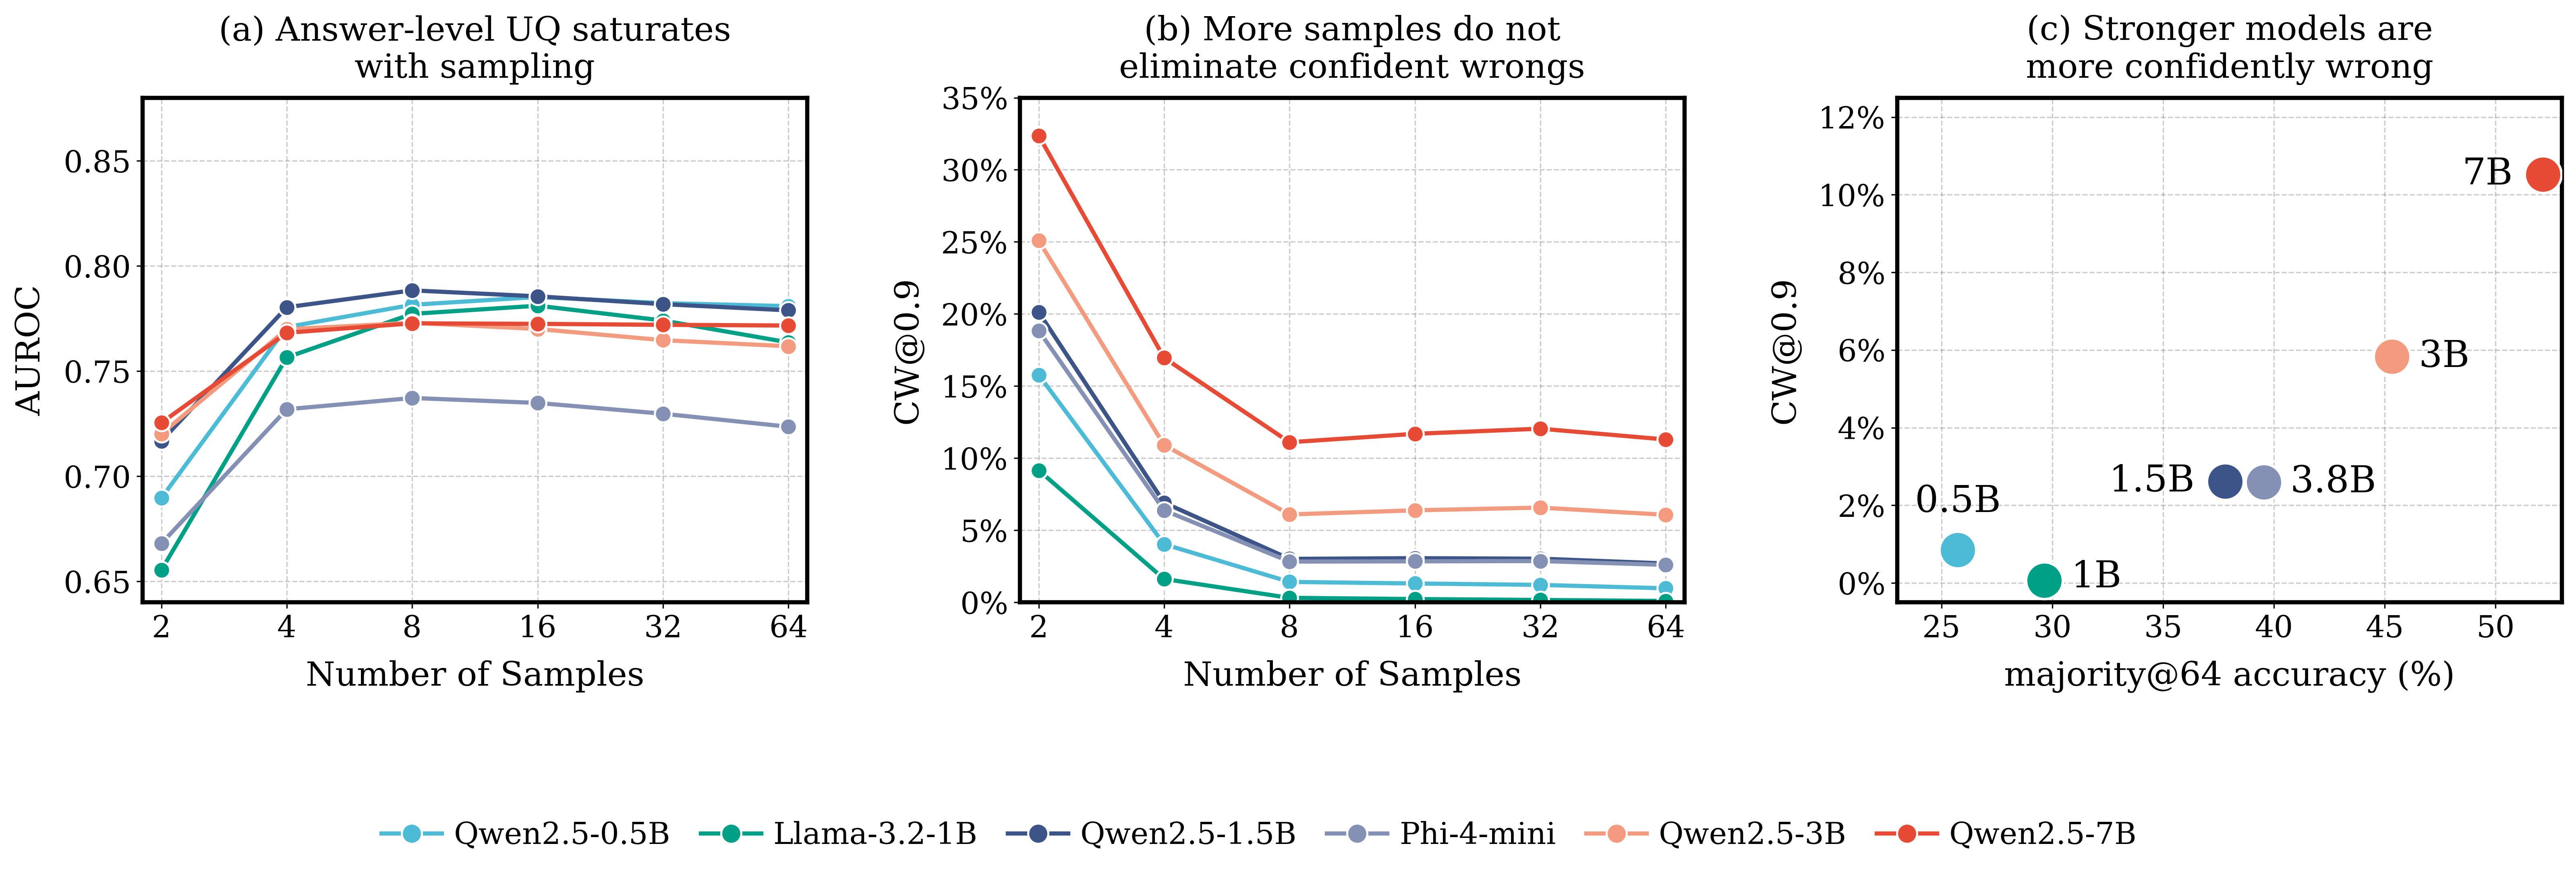
\includegraphics[width=\linewidth]{../../experiments/spurious_consensus/figures/fig_main.png}
    \caption{Extended SC failure-mode figure (six models, $K{=}64$). Panel (a): AUROC saturation; (b): CW@0.9 plateau; (c): capability vs.\ SCR.}
    \label{fig:app-sc-main}
\end{figure}

\begin{figure}[htbp]
    \centering
    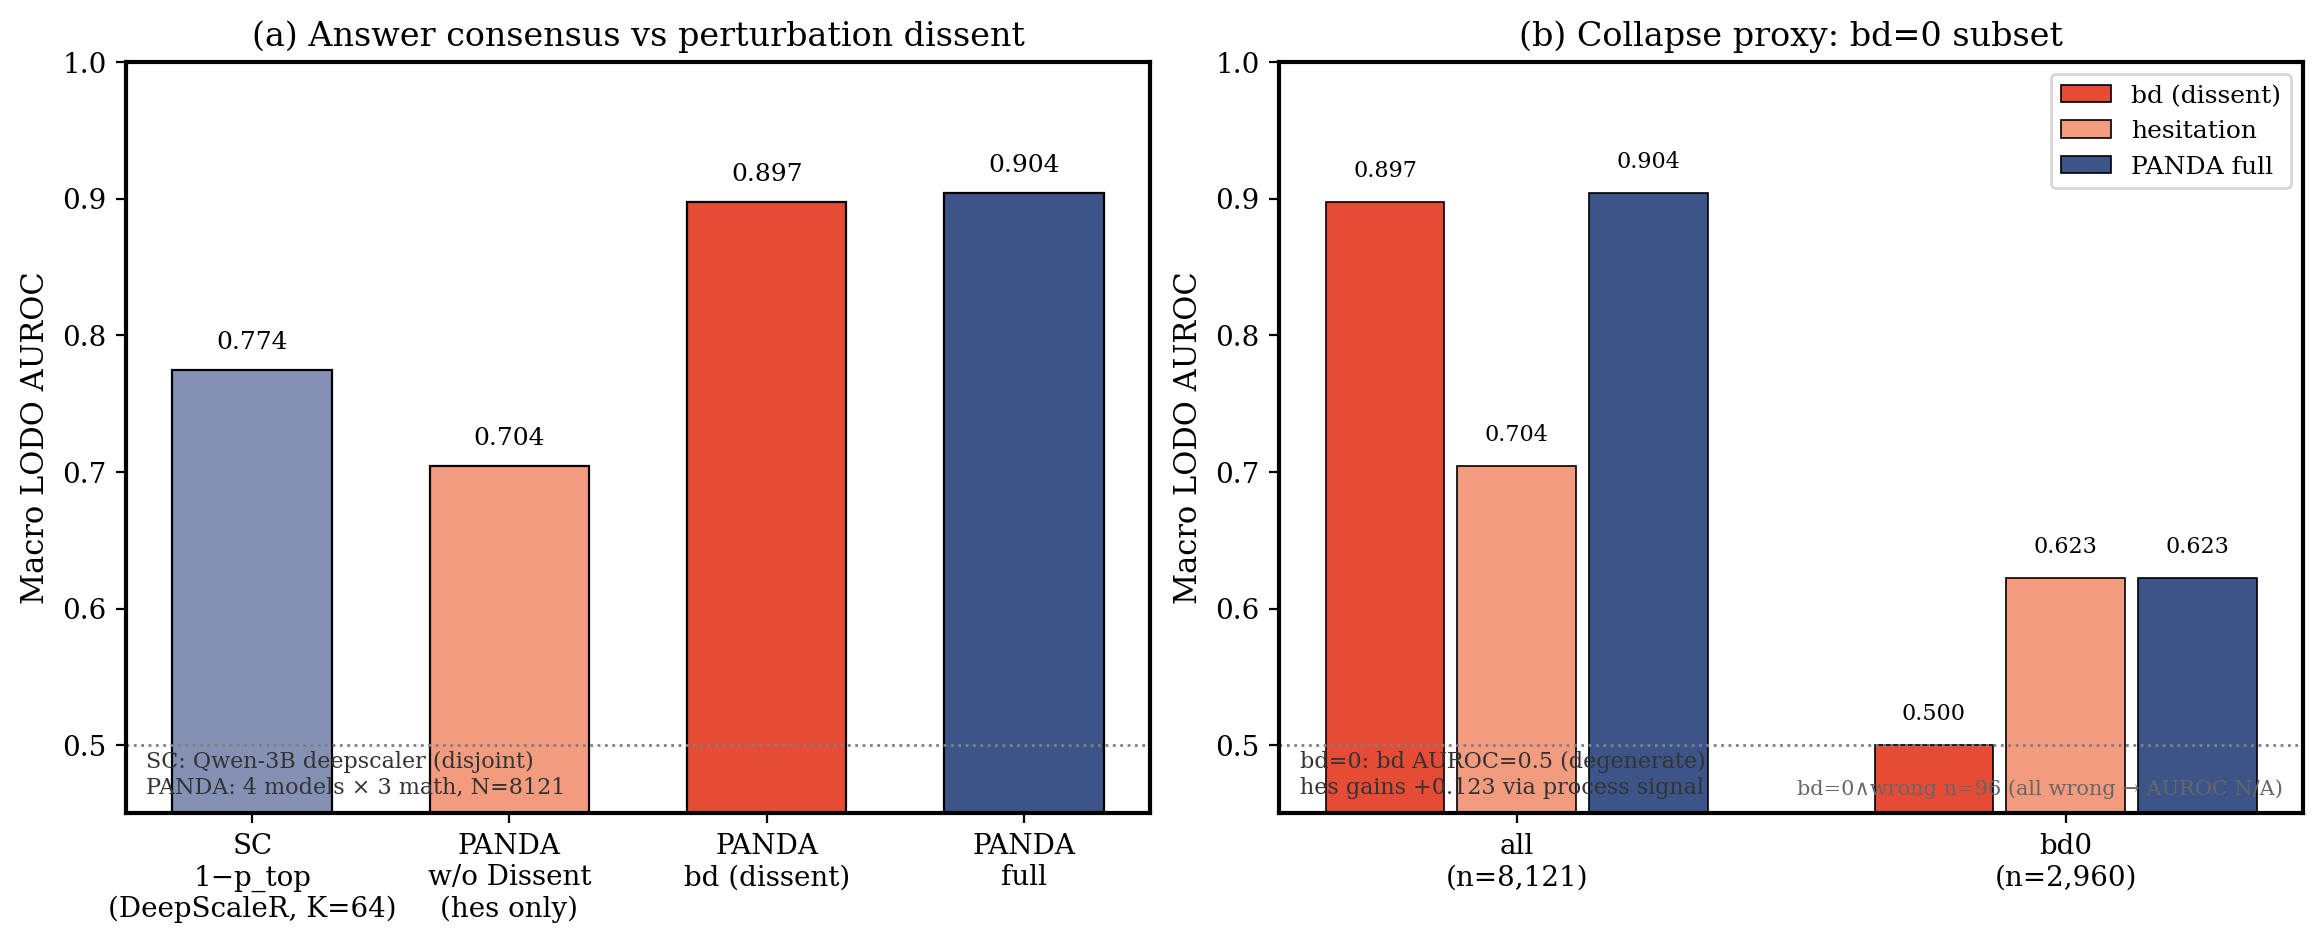
\includegraphics[width=\linewidth]{../analysis/figures/sc_vs_panda_dissent.png}
    \caption{Self-consistency dispersion vs.\ \method{} perturbation signals (CPU analysis; disjoint benchmark caveat in text).
    \textbf{(a)} Macro LODO AUROC: SC $1{-}p_{\mathrm{top}}$ on DeepScaleR (Qwen2.5-3B: 0.774) compared with \method{} and ablations on the main math cohort (full: 0.904; w/o Dissent: 0.704).
    \textbf{(b)} On the bd$=0$ collapse proxy ($n{=}2960$), dissent is uninformative (0.500) while hesitation remains at 0.623 (+0.123 AUROC over bd).}
    \label{fig:app-sc-vs-panda}
\end{figure}

\noindent\textbf{Caveat.} Panel (a) uses \emph{disjoint} benchmark sets (SC: DeepScaleR/GPQA/AIME; PANDA: Minerva/MATH-500/GSM8K) and should be read as complementary evidence rather than a paired per-question comparison.
On the small Minerva overlap ($n{=}198$), SC actually reaches higher AUROC (0.942 vs.\ 0.868 for dissent alone).


\section{Case Studies}
\label{app:cases}

\paragraph{Self-consistent collapse (SC).}
Consider a DeepScaleR word problem (id~12473) about Fox crossing a bridge: the gold answer is \textbf{25}, yet Qwen2.5-7B produces \textbf{220} in all 64/64 samples at $T{=}1.0$ (SCR@1.0).
The reasoning traces are \emph{not} copied verbatim---all 64 token sequences differ (average pairwise similarity 0.34)---yet they converge on the same incorrect template ($4\times50=200$ toll plus 20 coins left $\Rightarrow\boxed{220}$).
This is the hallmark of self-consistent collapse: diverse processes, unanimous wrong answer, and high token confidence (mean logprob $-0.088$).
Answer-level UQ based on $1-p_{\mathrm{top}}$ is blind here by construction.

\paragraph{Perturbation-caught drift and bd$=0$ remainder (\method{}).}
On our main math cohort, rephrasing-plus-weight perturbation shrinks the text-agreement wrong-rate proxy from 8.1\% to 3.2\% on bd$=0$ items, but 96 hard cases remain where every perturbation agrees with a wrong base answer.
These cases are distributed across models (Qwen2.5-3B: 38; Llama-3.2-1B: 28; Llama-3.1-8B: 24; Qwen3-8B: 6) and datasets (Minerva: 23; MATH-500: 34; GSM8K: 39).
Mechanism diagnostics show that near-answer proximity entropy $T_0$ alone does not predict failure (AUROC $\approx 0.50$), whereas dissent remains predictive even conditional on $T_0$ (residual AUROC 0.917).


\section{Baseline Fairness, TokUR Differentiation, and Cost}
\label{app:fairness}

\paragraph{Baseline fairness.}
All reported \method{} scores use out-of-fold logistic fusion without labels from the evaluated dataset.
Even the label-free fusion ablation (w/o Fusion: AUROC 0.877) remains above every standalone baseline in the macro average, confirming that the gains are not artifacts of in-set calibration.

\paragraph{TokUR EU differentiation.}
Compared with TokUR EU---a strong teacher-forced epistemic baseline that scores a \emph{fixed} greedy trace under weight perturbation---\method{} regenerates full responses under both prompt and weight probes and therefore captures answer-level reorganization that token-level epistemic variance may miss.
TokUR EU can still win on AUPRC in some low-error-rate cells (e.g., Llama-3.2-1B on Minerva: 0.979 vs.\ 0.954), where high class imbalance favors calibrated token uncertainty; \method{} instead prioritizes ranking wrong reasoning answers and improves AUROC/Acc@50 in most math settings.

\paragraph{Compute cost.}
Each question requires one greedy base decode, $R{=}4$ rephrase decodes, and $W{=}4$ weight-perturbed decodes ($\sim$9 generations), plus eight stochastic samples for the SE baseline.
Weight perturbations instantiate separate low-rank TFB model copies in memory during the weight branch.
The SC failure-mode study at $K{=}64$ uses a much larger budget (855k decodes across six models) and still leaves a confident-wrong residue.


\section{Reproducibility}
\label{app:repro}

\paragraph{Data and outputs.}
Raw per-sample records live under \texttt{panda-outputs/maintable\_\{model\}/seed\{S\}/raw\_runs/}.
Aggregated metrics: \texttt{paper/maintable/panda\_v2\_results.json}, \texttt{paper/analysis/cpu\_results.json}, and \texttt{paper/tables/mechanism\_results.json}.

\paragraph{Key scripts.}
\begin{itemize}[leftmargin=*, itemsep=2pt]
  \item Main-table generation: \texttt{scripts/run\_maintable\_3seed.sh}
  \item Aggregation: \texttt{scripts/aggregate\_prs\_v2.py}
  \item CPU paper analyses: \texttt{scripts/run\_cpu\_paper\_analyses.py}
  \item Mechanism / bd$=0$ studies: \texttt{scripts/analyze\_mechanism.py}, \texttt{scripts/analyze\_bd0\_subset.py}
  \item SC failure-mode figures: \texttt{experiments/spurious\_consensus/}
\end{itemize}


\section{Limitations}
\label{app:limitations}

Our evaluation focuses on verifiable-answer mathematical reasoning; open-ended generation is left to future work.
On the bd$=0$ subset where all perturbation runs agree with the base answer, Semantic Entropy can remain stronger than \method{} (0.708 vs.\ 0.623), and 96 hard collapse cases still lack rankable variance under dissent alone.
\method{} requires $\sim$9$\times$ decode overhead relative to a single greedy run, memory for multiple weight-perturbed model instances, and dependence on an external rephrasing API.
Extending \method{} to open-ended generation and designing more efficient perturbation schemes are promising directions for future work.

\end{document}
